\subsection{Data}
Table~\ref{tab:families} lists the seven shape families. Five are used for training: spheres (150 shapes), ellipsoids (350), capped cylinders
(300), tori (300) and smooth random blobs (900), the last being star-shaped surfaces built from six
low-frequency waves on the sphere. Two families are held out for testing only: superellipsoids (200),
with pointed tips or box-like rounded edges, and rough blobs (200), which add ten high-frequency waves.
Each shape is scaled to fill 35--100\% of the grid (diameters 9.8 to 60 voxels), randomly rotated and
shifted by a sub-voxel offset. The volume is formed by a simple CT model: partial-volume occupancy
computed with $5\times5\times5$ supersampling, a Gaussian blur with $\sigma=0.6$ voxel, and Gaussian noise
with $\sigma_n\in\{0, 0.05, 0.15\}$ relative to unit contrast, stored as 8-bit integers. Every shape is
rendered at $N=32$ and $64$ and all three noise levels, giving six volumes per shape and 14,400 in total.
The split is by shape (70/15/15 within each training family, fixed seed 51), so all six volumes of a
shape stay together: 1,400 training, 299 validation and 301 test shapes, plus the 400 held-out shapes.
Figure~\ref{fig:slices} shows one shape at both resolutions and all noise levels.

\begin{table*}[t]
  \centering\small
  \caption{Shape families. Parameters are drawn uniformly from the given ranges; all shapes are
  normalised to maximum extent 1 before placement.}
  \label{tab:families}
  \begin{tabular}{llrl}
    \toprule
    Family & Role & Shapes & Parameters \\
    \midrule
    Sphere & train & 150 & radius 1 \\
    Ellipsoid & train & 350 & $a=1$, $b,c\in[0.35,1]$ \\
    Cylinder (capped) & train & 300 & radius $\in[0.3,0.85]$, half-height $\sqrt{1-\rho^2}$ \\
    Torus & train & 300 & $r/R\in[0.2,0.6]$, $R+r=1$ \\
    Smooth blob & train & 900 & 6 waves, $\omega\in[1,3]$, s.d.\ of $\log r\in[0.15,0.30]$ \\
    \midrule
    Superellipsoid & held out & 200 & $b,c\in[0.45,1]$; $p\in[1.5,1.8]$ (40\%) or $[3,6]$ (60\%) \\
    Rough blob & held out & 200 & smooth blob $+$ 10 waves, $\omega\in[8,14]$, s.d.\ $\in[0.02,0.05]$ \\
    \bottomrule
  \end{tabular}
\end{table*}

\begin{figure}[t]
  \centering
  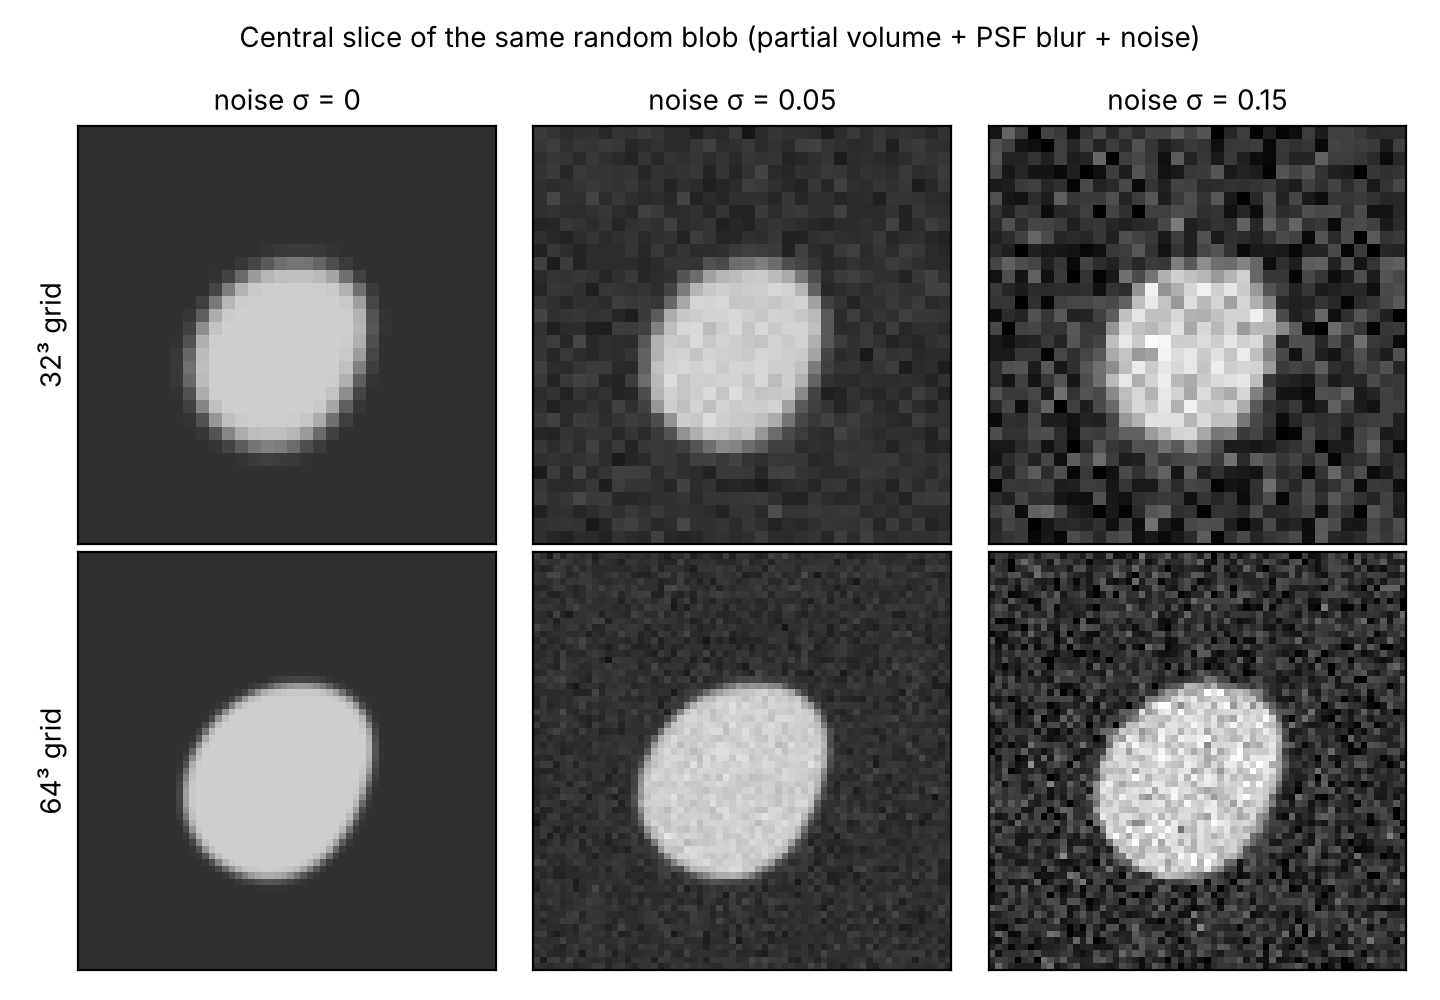
\includegraphics[width=\columnwidth]{example_slices.png}
  \caption{Central slice through the same random blob at both resolutions and all three noise levels.}
  \label{fig:slices}
\end{figure}

\begin{figure}[t]
  \centering
  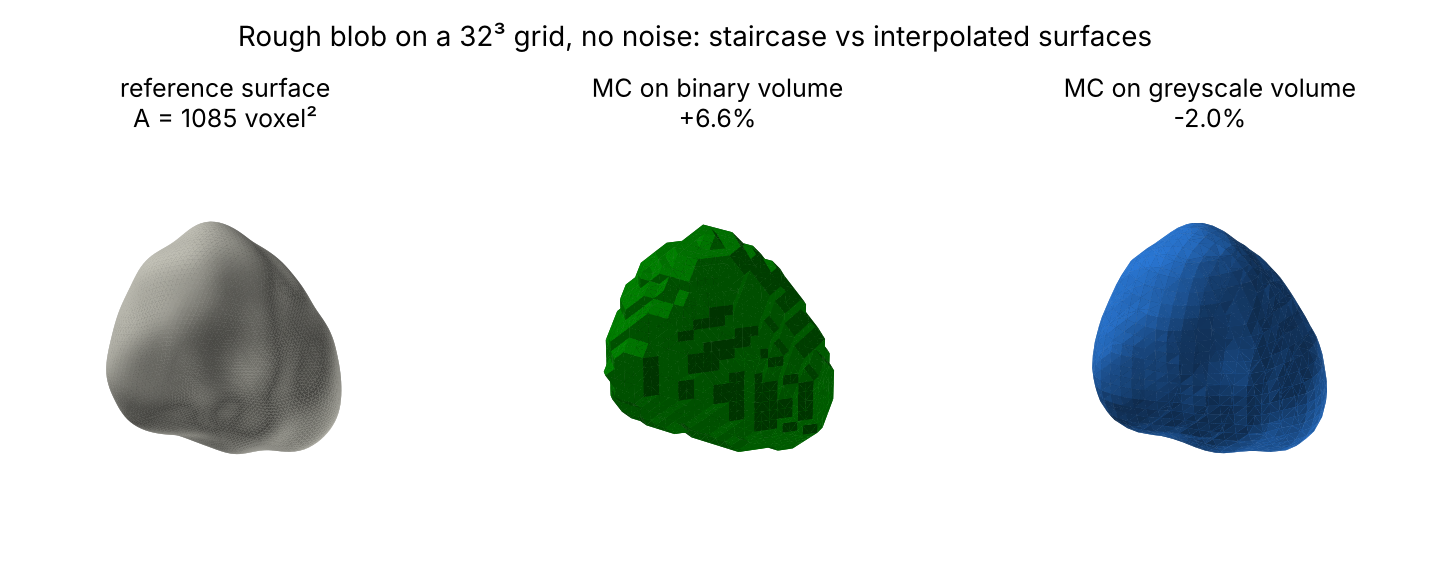
\includegraphics[width=\columnwidth]{example_meshes.png}
  \caption{Reference surface of a rough blob and the marching-cubes meshes from its clean $32^3$ volume.
  The binary mesh is a staircase; the greyscale mesh is smooth but loses the finest detail.}
  \label{fig:meshes}
\end{figure}

\subsection{Estimators}
\textbf{Classical:} voxel-face counting after thresholding at 0.5; marching cubes on the thresholded
(binary) volume; marching cubes on the greyscale volume at iso-level 0.5; and marching cubes after
Gaussian smoothing with $\sigma_s=1$ voxel (Fig.~\ref{fig:meshes}). \textbf{MC + lookup} multiplies the
greyscale area by the median training correction for the same resolution and noise level; it is given
the true noise level, so any learned model has to beat it to show that it does more than apply an
average. \textbf{Random Forest} \citep{breiman2001} (400 trees) predicts $y$ from ten simple
measurements: the greyscale area relative to $N^2$, the ratios of the face, binary and smoothed areas to
it, a compactness term, two aspect ratios, the Euler number of the thresholded volume, a noise estimate
and $N$.

\textbf{3D CNN:} five convolutional blocks with 16 to 256 channels, batch normalisation, ReLU and max
pooling, then global average and max pooling and a 128-unit head (3.59M parameters).
\textbf{PointNet} \citep{qi2017}: 2,048 points sampled on the greyscale mesh, a shared MLP up to 1,024
features, max pooling and a 512--128 head (0.74M parameters), with random rotations instead of the
alignment network. Both are trained per resolution with a Huber loss on $y/0.05$, AdamW, a one-cycle
learning-rate schedule \citep{smith2019} with peak $10^{-3}$, batch size 32, up to 40 epochs (15 for the
CNN at $64^3$) and early stopping on the validation error, using PyTorch \citep{paszke2019} on an
Apple-silicon laptop. We report the mean absolute percentage error (MAPE) and the mean signed error
(bias) of $\hat A/A_\text{true}-1$ on held-out shapes only.
